\begin{figure}[t]
\centering
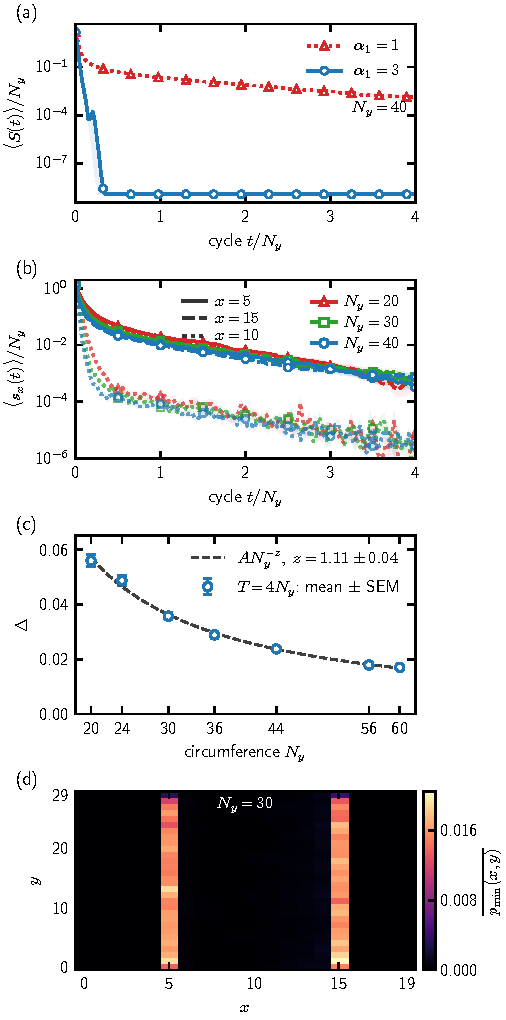
\includegraphics[width=\columnwidth]{hard_wall_purification_contours_gap_density_4x1.pdf}
\caption{Hard-wall purification from a maximally mixed active slab:
$N_x=20$, $\alpha_2=30$, $n_{\rm shell}=1$, perfect correction,
100 independent Born trajectories per configuration, and $T=4N_y$.
(a) Mean entropy at $N_y=40$ for $\alpha_1=1,3$.
The near-zero control tail is the numerical entropy floor.
(b) Column contours at $\alpha_1=1$, summed over $y$ and orbitals,
for $N_y=20,30,40$. Bands denote one sample SEM.
(c) Mean endpoint gap $\Delta=\min_j|\lambda_j|$, with
$\lambda_j=-\operatorname{atanh}(a_j)/T$, centered covariance
eigenvalues $a_j$, and SEM bars. The all-size power-law fit gives
$\Delta\propto N_y^{-1.11\pm0.04}$.
(d) At $N_y=30$, $\alpha_1=1$, the orbital-summed probability
density of the single smallest-$|\lambda_j|$ eigenmode is selected
separately in each trajectory, then averaged over 100 trajectories.
All selected minima are nondegenerate. The mean density sums to one;
colors are linear.}
\label{fig:hard-wall-purification-control}
\end{figure}
